\chapter{Introduzione alle carte raster}

\section{Importare una carta raster\label{sec:Importare-una-carta}}
	L'importazione di carte raster avviene con lo stesso procedimento adottato per le carte vettoriali, che si vedrà successivamente in \textsection\ref{sub:Importare-un-file-dxf}. L'importazione vera e propria viene effettuata tramite una delle voci del menù \textsf{$\text{File}\rightarrow\text{Import~raster~map}$} a seconda della tipologia di raster da importare. La soluzione più conveniente per i normali normali formati raster (ad esempio png, jpeg, tiff e geotiff, georeferenziati e non) è comunque quella di usare le funzioni offerte dalla libreria GDAL.

	\begin{itemize}
		\item creare una nuova location con sistema di riferimento XY;
		\item dopo averla avviata, dal Layer Manager selezionare \textsf{$\text{File}\rightarrow\text{Import~raster~map}\rightarrow\text{Import~raster~data~using~GDAL}$}, aprendo l'interfaccia grafica del modulo \textsf{r.in.gdal};
		\item nella scheda \textsf{Required} occorre selezionare il file da importare e il nome del rispettivo layer;
		\item non appena definite le varie opzioni (ricordandosi eventualmente di spuntare l'opzione in basso \textsf{Add created map into layer tree}), fare click su \textsf{Run}; nel \textsf{Command output} è possibile seguire lo stato dell'importazione e leggere le segnalazioni di eventuali errori.
	\end{itemize}

			\paragraph{Semplificare l'importazione di molti layer raster}
				Esiste una maniera semplice per importare più file raster in layer differenti, la voce di menù \textsf{$\text{File}\rightarrow\text{Import~vector~map}\rightarrow\text{Multiple~raster~data~import}$}, facente sempre capo al modulo \textsf{r.in.gdal}. Selezionandola, si aprirà una finestra in cui è possibile selezionare la cartella che contiene i file da importare, scremati per estensione (che deve essere preventivamente indicata nella casella \textsf{Select file extensions}.

\section{\label{sec:Georeferenziare-una-carta-raster}Georeferenziare una carta raster}
	Adesso che abbiamo ottenuto una location con una mappa posizionata in un sistema di riferimento XY, è possibile georeferenziarla, ovvero trasferirla dalla location corrente ad una già georiferita, che è caratterizzata anche da un sistema di riferimento spaziale (nel nostro caso UTM - WGS84). L'operazione (riassunta in fig.~\ref{fig:georef}) viene svolta utilizzando le funzioni del modulo \emph{i.vpoint}, che permette di assegnare ad alcuni punti della carta raster le coordinate geografiche prese dallo stesso punto su una carta già georeferenziata (raster o vettoriale). Per fare ciò è possibile avvalersi di quattro diversi moduli di GRASS: \emph{i.group}, \emph{i.target}, \emph{i.vpoints}, \emph{i.rectify}.
	
	\begin{description}
		\item [{\emph{i.group}}] crea, modifica e cancella gruppi di immagini raster, anche in più livelli, per facilitarne la gestione e le eventuali operazioni in blocco;
		\item [{\emph{i.target}}] indirizza un certo gruppo di immagini verso una ben precisa location e mapset;
		\item [{\emph{i.vpoints}}] registra i punti di controllo su un certo gruppo di immagini, permettendo di associarli a coordinate prelevate da una mappa vettoriale o raster già georeferenziati;
		\item [{\emph{i.rectify}}] rettifica un'immagine calcolando la trasformazione di coordinate per ogni pixel dell'immagine da georeferenziare, basandosi sui punti di controllo registrati con \emph{i.vpoints}.
	\end{description}

	\begin{figure}
		\centering
		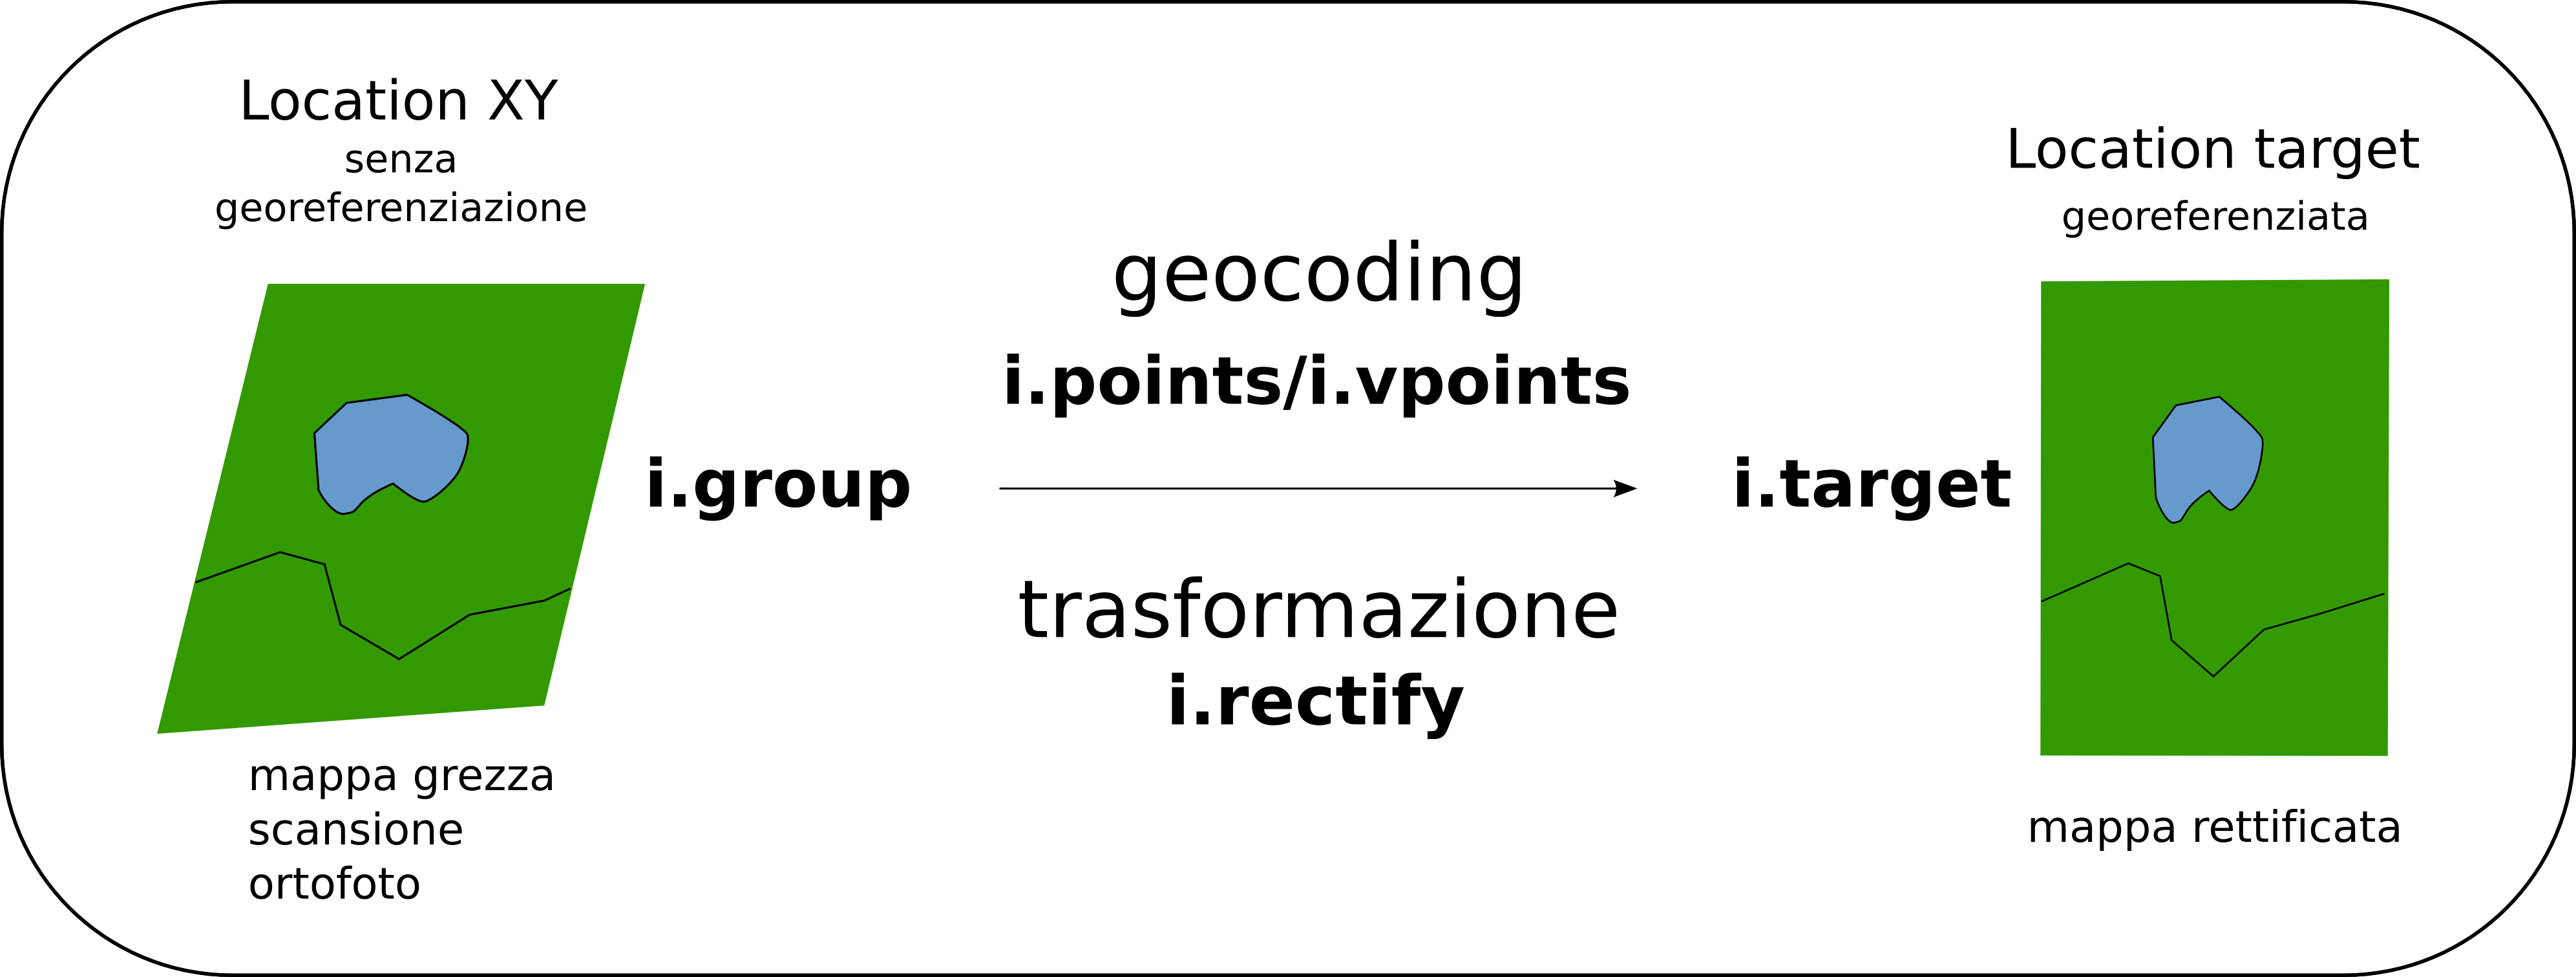
\includegraphics[scale=0.35]{img/g4556}
		\caption{{\small \label{fig:georef}Schema riassuntivo dei moduli coinvolti nel processo di georeferenziazione di una carta vettoriale o raster.}}
	\end{figure}

	\subsection{Gruppi e target}
		Considerato che GRASS è stato progettato per essere flessibile e lavorare con quantità variabili di dati, i moduli \emph{i.group} ed \emph{i.target} permettono di gestire il ``movimento'' dei dati mentre si effettua un'operazione su di essi. Nel caso della georeferenziazione, permettono di creare un gruppo di una o più mappe raster non georiferite e, dopo tale processo, di muoverle verso il target, che è la location (ed il rispettivo mapset) di destinazione, caratterizzati entrambi da un preciso sistema di riferimento. In breve, prima di georeferenziare qualsiasi immagine, è necessario importarla in una location con un sistema di riferimento XY, quindi inserirla in un gruppo (creandolo, se necessario), e definire come target location il mapset di destinazione (nel nostro caso quello del sito archeologico del quale sono già state definite le caratteristiche cartografiche precedentemente).

		\subsubsection{Creare e gestire un gruppo}
			Si ipotizzi di avere la location XY \emph{immagini} contenente (all'interno del proprio mapset di base, \emph{PERMANENT}), una mappa raster dell'Istituto Geografico Militare (IGM) denominata \emph{siponto\_IGM}, e di volerla georeferenziare ed inserire nella location \emph{siponto}, nel suo mapset di base (\emph{PERMANENT}).
			
			\begin{enumerate}
				\item Accedere a GRASS ed avviare la location contenente il mapset dell'immagine da georeferenziare (\emph{immagini}); è essenziale che il gruppo sia creato all'interno della location che contiene l'immagine da elaborare, non nella location di destinazione.
				\item Dal menù selezionare \textsf{$\text{Imagery}\rightarrow\text{Develop~images~and~groups}\rightarrow\text{Create/edit~group}$}; nella finestra appena aperta è necessario inserire nella scheda \textsf{Required} il nome per il nuovo gruppo (nel nostro esempio \emph{carte\_IGM}); nella scheda \textsf{Optional} è possibile definire, nell'ultimo menù a tendina, quali immagini di mappe raster inserire nel gruppo. È possibile selezionarne anche molteplici, ma in questa prima importazione è disponibile solo la mappa \emph{siponto\_IGM}.
				\item Fare quindi click su \textsf{Run}. La carta \emph{siponto\_IGM} viene inserita nel gruppo \emph{carte\_IGM}, e veniamo avvisati dal programma che l'operazione è andata a buon fine, con il seguente output:\\

				\begin{verbatim}
					Adding raster map <siponto_IGM@PERMANENT> to group i.group complete.
				\end{verbatim}
			
				\item Per inserire un'altra mappa nello stesso gruppo, ripetere l'operazione dal punto 1, selezionando nella scheda \textsf{Required} il nome del gruppo già creato, senza digitarne uno nuovo.
			\end{enumerate}

			\input{tab/box_gestire_carte}
			
		\subsubsection{\label{sub:Definire-un-target}Definire un target}
			Per definire una location target alla quale destinare il risultato dell'elaborazione di un certo gruppo, procedere come segue (dopo aver eseguito l'istruzione 1 della sezione precedente):
			
			\begin{enumerate}
				\item Dal menù selezionare \textsf{$\text{Imagery}\rightarrow\text{Develop~images~and~groups}\rightarrow\text{Target~group}$}; nella finestra appena aperta è necessario selezionare nel menù a tendina nella scheda \textsf{Required} il nome del gruppo (precedentemente creato) che si vuole ``indirizzare'' verso il target; nell'esempio il gruppo creato era chiamato \emph{carte\_IGM@PERMANENT}.
				\item Nella scheda \textsf{Optional} bisogna definire la location ed il mapset di destinazione, scrivendoli rispettivamente nei campi \textsf{Name of imagery target location:} e \textsf{Name of target mapset:}; nell'esempio, il gruppo \emph{carte\_IGM@PERMANENT}i deve essere inserito, dopo la georeferenziazione, nella location \emph{siponto} e nel mapset \emph{PERMANENT}, quindi:

				\begin{verbatim}
					Name of imagery target location: siponto
					Name of target mapset: PERMANENT
				\end{verbatim}
				
				\item Al termine dell'operazione, fare click su \textsf{Run}. Si otterrà un output simile al seguente:

				\begin{verbatim}
					i.target group=carte_IGM@PERMANENT location=siponto mapset=PERMANENT
					Group <carte_IGM> targeted for location [siponto],
					mapset [PERMANENT] i.target complete.
				\end{verbatim}
			\end{enumerate}

	\subsection{Registrare i punti di controllo}
	
		\begin{itemize}
			\item Avviare GRASS nella location in cui è presente la mappa raster non georiferita, nel sistema di riferimento XY (nel nostro esempio, \emph{immagini}).
			\item Tornare nella finestra di terminale per avviare una nuova sessione grafica di lavoro, ovvero un nuovo ``monitor'':

			\texttt{d.mon x0}

			In seguito a tale comando si aprirà una finestra, inizialmente a sfondo bianco, all'interno della quale verranno eseguite le funzioni del modulo \emph{i.vpoint}s, che serve a registrare i punti di controllo al suolo (\emph{ground control points}, abbr. \emph{GCP}) su entrambe le mappe, ovvero i riferimenti in base ai quali la mappa verrà georeferenziata\footnote{Una valida alternativa al comando \emph{i.vpoints} è \emph{i.point}s, con l'unica differenza che il primo supporta, nel corso delle operazioni, il caricamento anche di mappe vettoriali da usare come riferimento per la georeferenziazione.}.

			\item Prima di eseguire il modulo \emph{i.vpoint}, è necessario sapere che è possibile indicare direttamente quale gruppo di immagini deve essere georeferenziato, semplicemente facendo seguire al comando \texttt{i.vpoints} il nome del gruppo di immagini (precedentemente creato) che si vuole georeferenziare; nel nostro esempio:

			\texttt{i.vpoints carte\_IGM}

			\end{itemize}

			\input{tab/box_immagini_georef}
			
			\begin{itemize}
				\item Si aprirà quindi nella finestra della grafica, fin'ora bianca, un menù che chiede di fare doppio click sulla carta da georeferenziare (vengono elencate tutte quelle presenti nel gruppo indicato --- nel nostro caso \emph{carte\_IGM}). Verrà quindi caricata nel riquadro in alto a sinistra la carta selezionata.
				\item Facendo attenzione, si noterà nella parte inferiore della finestra in cui è presente la carta, una serie di comandi; tali controlli permettono di gestire la mappa caricata:

				\begin{description}
					\item [{\textsf{QUIT}}] esce dal modulo \emph{i.vpoint}s;
					\item [{\textsf{ZOOM}}] permette di effettuare lo zoom sulla mappa, spesso indispensabile su carte raster molto ampie; comprende le seguenti funzioni:

					\begin{description}
						\item [{\textsf{BOX}}] effettua lo zoom su un'area dell'immagine, selezionabile facendo click e trascinando con il tasto sinistro del mouse; 
						\item [{\textsf{POINT}}] effettua lo zoom su un punto, permettendo di impostare manualmente il livello di ingrandimento.
					\end{description}
				\item [{\textsf{RASTER}}] permette di selezionare un altro file di mappa raster al posto di quello corrente;
				\item [{\textsf{VECTOR}}] permette di aprire una carta vettoriale dalla quale prelevare le coordinate da associare ai punti di controllo.
				\end{description}
				
				Gli altri comandi disponibili per il momento non sono utilizzabili, verranno analizzati successivamente.

				\item Nei due riquadri a sinistra (in alto e in basso) vengono visualizzati i due livelli di ingrandimento della mappa da georeferenziare, mentre nei due riquadri sulla destra della finestra è possibile caricare un'altra mappa (raster o vettoriale) già georeferenziata da usare come riferimento. Per farlo, selezionare a seconda delle necessità \textsf{Raster}\footnote{Se si seleziona \textsf{Raster} verrà chiesto dal programma in quale lato della finestra \emph{plottare} la carta; fare click sul riquadro in alto a destra.} o\textsf{$\text{Vector}\rightarrow$}\textsf{\emph{Carta~georeferenziata}}.
				
				\item Dopo aver usato lo zoom nelle due mappe per posizionare i due display nella stessa zona, fare click con il tasto sinistro prima sul punto della carta da georeferenziare e poi su quello della carta georeferenziata; in questo modo al punto della prima carta verranno associate le coordinate del punto della seconda carta, a noi note.\\

				Alternativamente a questo punto, è possibile anche che si abbiano già a disposizione le coordinate di alcuni punti e non ci sia bisogno di cercare il raffronto con una carta raster o vettoriale già georeferenziata; ad esempio, è possibile che il raster che si sta cercando di georeferenziare sia la scansione di una mappa cartacea, nel qual caso saranno note le coordinate dei quattro angoli della carta, o delle intersezioni tra meridiani e paralleli. In questa situazione:
				
				\begin{itemize}
					\item fare semplicemente click con il tasto sinistro sul punto del raster di coordinate note;
					
					\item osservando il terminale si noterà che vengono visualizzate le coordinate del raster in quel punto, ed è possibile inserire latitudine e longitudine del punto segnalato (in particolare, verrà chiesta prima la longitudine N e poi la latitudine E), separati semplicemente da uno spazio\footnote{In questo frangente è possibile anche convertire al volo le coordinate del punto in esame in un altro sistema di riferimento, ed inserirle già convertite, utilizzando la procedura che verrà descritta in \textsection\ref{sec:Coordinate-ellissoidiche-e}.}; 
					
					\item dopo aver premuto \textsf{Invio} verrà chiesta conferma con la pressione del tasto \textsf{y}.
				
						
				\end{itemize}

				\item Dopo aver ripetuto l'operazione per almeno altre due volte (segnando quindi un minimo di due punti), è possibile procedere con lo strumento di analisi, avviabile tramite il pulsante \textsf{Analyze}. Apparirà un riquadro grigio con l'elenco dei punti raccolti.
			
			\end{itemize}

			\input{tab/box_quanti_punti}
			
			\begin{itemize}
				\item L'elenco dei punti raccolti presenta 3 coppie di colonne:

				\begin{description}
					\item [{\textsf{error}}] presenta l'errore nell'individuazione dei punti, sull'asse delle ascisse e delle ordinate;
					\item [{\textsf{image}}] presenta le coppie di coordinate cartesiane prese sulla mappa non georeferenziata (infatti i valori sono espressi in ``celle'');
					\item [{\textsf{target}}] presenta i corrispondenti valori di coordinate definite sulla base del sistema di riferimento utilizzato nella mappa georeferenziata (in questo caso, UTM WGS 84).
				\end{description}
				
				Facendo doppio click su una delle righe presentate, il punto viene escluso dal calcolo. Per agevolare la scelta, vengono presentati in rosso i punti che presentano un errore più alto. È quindi chiaro che anche in vista di una trasformazione di primo grado, per la quale sono necessari solo 3 punti, è sempre utile selezionarne qualcuno in più, per poi escludere quelli con maggior errore. Perché la trasformazione avvenga correttamente, è bene selezionare punti ai quattro angoli della mappa da georeferenziare, distanziandoli il più possibile.

				\item Premendo il pulsante \textsf{Overlay} è possibile sovrapporre le due mappe, per osservare se coincidono. Se il risultato è soddisfacente, premere \textsf{Done} per ritornare al monitor principale. \textsf{Quit} terminerà il modulo.
			\end{itemize}

	\subsection{Rettificare e georeferenziare la carta}
		Per procedere ai passi finali della georeferenziazione, è necessario usare il modulo \emph{i.rectify}, accessibile dal layer manager di GRASS, tramite il menù \textsf{$\text{Imagery}\rightarrow \text{Rectify image or raster.}$} Nella maschera che appare, selezionare il nome del gruppo di immagini su cui si è lavorato fin'ora (\textsf{Name of input imagery group}), e inserire nella seconda casella di testo il suffisso da applicare al nome delle mappe rettificate (ad esempio, \texttt{\_rect}). Nell'ultima casella di testo, \textsf{Rectification polynom order (1-3)} inserire il numero dell'ordine del polinomio di rettifica, precedentemente selezionato, quindi premere su \textsf{Run}. Il processo di rettifica e georeferenziazione, al termine, copierà le nuove mappe georeferenziate e rinominate nella location target (definita in \textsection\ref{sub:Definire-un-target}, nel nostro caso \textsf{siponto}).

		Per osservare il risultato, chiudere GRASS e riaprirlo nella location target. Se il risultato è soddisfacente e le mappe raster non georeferenziate non sono più di alcuna utilità, è auspicabile ritornare nella location con sistema di riferimento XY che contiene le immagini non georeferenziate e cancellarle, per risparmiare spazio su disco.


\section{Riproiettare una carta raster\label{sec:Riproiettare-raster}}
	Può accadere di essere in possesso di dati ottenuti da varie fonti (da enti che li distribuiscono, ad esempio) già georeferenziati, ma in un sistema di riferimento differente da quello con il quale si è soliti lavorare o diverso da quello previsto dal progetto in opera.  Per mantenere l'omogeneità del lavoro, senza doverlo georeferenziare nuovamente (con tutti gli inconvenienti del processo), è sufficiente riproiettarlo utilizzando le funzioni del modulo \texttt{r.proj}.  Prima di procedere, occorre avere:
	
	\begin{itemize}
		\item i dati da riproiettare già presenti in una propria location (in questo esempio, Gauss-Boaga fuso est, EPSG 3004, a cui è stato dato nome \texttt{location-boaga});
		\item una location di destinazione in cui è stato impostato il sistema di riferimento ``finale'' (nell'esempio UTM WGS84, a cui è stato dato nome \texttt{location-WGS}).
	\end{itemize}
	
	Il modulo \texttt{r.proj} presenta un inconveniente: l'estensione della region di destinazione deve essere sufficientemente ampia da poter contenere il raster riproiettato; in caso contrario, si otterrà un errore del genere:
	
	\begin{verbatim}
		ERROR: Input raster map is outside current region
	\end{verbatim}
	
	Un utile metodo è quello di creare nella location di partenza un dato vettoriale ``fittizio'' delle esatte dimensioni del raster da riproiettare, e riproiettarlo usando \texttt{v.proj} nella location destinazione (fortunatamente il programma vettoriale non ha problema di contenimento della region); quindi adattare la region al vettore risultante, per poi procedere alla riproiezione del raster. Procedere come segue.
	
	\begin{enumerate}
		\item Nella location di partenza, in cui è presente la carta da riproiettare, ridimensionare la region in base all'estensione del raster e creare un vettore esattamente di tale dimensione tramite l'apposito modulo \texttt{v.mkgrid} (\texttt{mio\_raster} è il nome del raster da georeferenziare, \texttt{vettore\_estensione} è il nome del vettore grande quanto il raster, a cui può essere attribuito un nome casuale):

		\begin{verbatim}
			g.region -p rast=mio_raster
			v.mkgrid map=vettore_estensione grid=1,1 position=region
		\end{verbatim}
		
		\item Nella location di destinazione, riproiettare ed importare il vettore, e ridimensionare la region della location in base a questo:

		\begin{verbatim}
			v.proj location=location-gauss mapset=PERMANENT in=vettore_estensione
			g.region vect=vettore_estensione+
		\end{verbatim}
	
		\item Adesso che la region è stata ridimensionata ad una grandezza sufficiente per poter importare il raster, è possibile procedere con la riproiezione e importazione della carta:

		\begin{verbatim}
			r.proj location=location-gauss mapset=PERMANENT in=mio_raster res=risoluzione
		\end{verbatim}
	\end{enumerate}

\section{Definire i colori}
	In GRASS, i colori sono definiti usando la codifica RGB (\emph{Red, Green, Blue}), ciò significa che ogni colore è identificato da una terna di valori, ognuno dei quali rappresenta una gradazione dei tre colori fondamentali rosso, verde e blu, espressi in una scala di intensità che va da 0 a 255. Ad esempio, il verde sarà composto dai valori R=0, G=255, B=0.
	
	I colori di una carta raster si ottengono associando ad ogni valore numerico del raster una terna di questi valori; i colori della carta vengono salvati in un file di testo che ha lo stesso nome del file raster a cui è associato, presente nella cartella \texttt{\emph{grassdata}}\texttt{/}\texttt{\emph{location}}\texttt{/colr}.

	È possibile inoltre associare:
	
	\begin{itemize}
		\item un colore per ogni valore del raster;
		\item definire un intervallo di valori tra tutti i valori del raster ed associare un colore solo agli estremi di tale intervallo; in tal caso i colori intermedi sono calcolati da GRASS interpolando i tre valori RGB associati agli intervalli.
	\end{itemize}
	
	Si noterà che nonostante non si sia definito manualmente alcun colore per le carte raster già importate, esse sono comunque colorate, poichè GRASS associa di default una colorazione. Ciò può provocare dei problemi a livello di lettura della carta quando si affiancano due carte raster che hanno differenti valori di massimo e minimo (ad esempio dell'altitudine in tue tasselli di una carta altimetrica che rappresentano uno la pianura e l'atro il rilievo), che avranno scale di colori simili a livello estetico ma diverse in fase di lettura. Nasce quindi la necessità di definire scale di valori omogenee per due o più carte; ipotizzando che si voglia lavorare su due carte, per farlo è necessario:
	
	\begin{enumerate}
		\item conoscere i valori minimi e massimi di entrambe le carte:

		\begin{enumerate}
			\item caricare entrambe le carte nel layer manager;
			\item avviare il modulo \textsf{r.info} dal menù \textsf{$\text{Raster}\rightarrow\text{Report~and~statistics}\rightarrow\text{Basic~raster~metadata}$}; nella scheda \textsf{Required} selezionare una delle due carte, e prima di premere \textsf{Run} selezionare l'opzione \textsf{Print range only} nella scheda \textsf{Optional};
			\item i valori di minimo e massimo relativi al raster selezionato dovrebbero apparire accanto alle voci \texttt{min} e \texttt{max}:

			\begin{verbatim}
				min=-2
				max=873
			\end{verbatim}
		
			\item ripetere il punto precedente con l'altra carta;
		\end{enumerate}
		
		\item definire la tabella dei colori per uno dei due raster:

		\begin{enumerate}
			\item avviare il gestore dei colori dal menù \textsf{$\text{Raster}\rightarrow\text{Manage~colors}\rightarrow\text{Color~rules}$};
			\item dalla casella in basso è possibile aggiungere un nuovo valore della carta (non necessariamente compreso tra il minimo e il massimo della mappa selezionata) al quale attribuire un colore;
			\item definire un intervallo di valori che comprendano il minimo e il massimo delle successive carte che si vogliono comprendere nella colorazione;
		\end{enumerate}

		\item applicare la medesima tabella anche all'altro raster:

		\begin{enumerate}
			\item avviare il gestore delle tabelle dei colori dal menù \textsf{$\text{Raster}\rightarrow\text{Manage~colors}\rightarrow\text{Color~tables}$};
			\item nella scheda \textsf{Required} selezionare l'altra carta non ancora colorata;
			\item recarsi nella scheda \textsf{Optional} e impostare nel campo \textsf{Raster map name from which to copy the table} la carta dalla quale la tabella dei colori dovrà essere copiata, quindi avviare il comando con \textsf{Run}.
		\end{enumerate}
	\end{enumerate}
